\subsection{Wiener measure}

In this No., we denote by T the interval \([0,1]\) of R and by H the Hilbert space of real functions on T square-integrable with respect to Lebesgue measure, where the scalar product is denoted \((f|g)\) . We also denote by C the space of continuous real functions on T tending to 0 at the point 0; we equip C with the norm \(\|f\| = \sup_{t \in T} |f(t)|\) . The compact interval \([0,1] = T \cup \{0\}\) is the Alexandroff compactification of the locally compact but noncompact interval T; consequently, the set of continuous functions on T with compact support is dense in C, and the dual of C may be identified with the space \(M^{1}\) of bounded measures (not necessarily positive) on T (Ch. III, §1, No.~8, Def. 3).

For every function \(f \in \mathcal{H}\) , one defines a function \(Pf\) on \(T\) by

\[
(P f) (t) = \int_ {0} ^ {t} f (x) d x = (f | \mathrm{I} _ {t}),\tag{31}
\]

where \(I_{t}\) is the characteristic function of the interval \([0, t]\) . The Cauchy--Schwarz inequality implies the inequalities

\[
| (P f) (t) | \leqslant \| f \| _ {2} \cdot t ^ {1 / 2}\tag{32}
\]

\[
\left| (P f) (t) - (P f) \left(t ^ {\prime}\right) \right| \leqslant \| f \| _ {2} \cdot \left| t - t ^ {\prime} \right| ^ {1 / 2}\tag{33}
\]

consequently, \(Pf\) belongs to \(\mathcal{C}\) , and the linear mapping \(P\) of \(\mathcal{H}\) into \(\mathcal{C}\) is continuous with norm \(\leqslant 1\) .

Let us identify the Hilbert space \(\mathcal{H}\) with its dual (TVS, V, §1, No.~7, Th. 3), and denote by \(\Pi : \mathcal{M}^1 \to \mathcal{H}\) the transpose of \(P: \mathcal{H} \to \mathcal{C}\) . For every measure \(\mu \in \mathcal{M}^1\) and every function \(f \in \mathcal{H}\) , we have

\[
\begin{array}{r l} (\Pi \mu | f) & = \mu (P f) = \int_ {\mathrm{T}} d \mu (t) \int_ {\mathrm{T}} \mathrm{I} _ {t} (x) f (x) d x \\ & = \int_ {\mathrm{T}} f (x) d x \int_ {\mathrm{T}} \mathrm{I} _ {t} (x) d \mu (t) \end{array}
\]

by the Lebesgue--Fubini theorem. Now,

\[
\mathrm{I} _ {t} (x) = \left\{ \begin{array}{l l} 1 & \text { if } 0 <   x \leqslant t \leqslant 1 \\ 0 & \text { otherwise }, \end{array} \right.
\]

whence finally

\[
(\Pi \mu) (x) = \mu ([ x, 1 ]) \quad \text { for } x \in \mathbf {T}.\tag{34}
\]

Let \(\mu, \nu\) be in \(\mathcal{M}^1\) . Then

\[
\begin{array}{r l} (\Pi \mu | \Pi \nu) & = \int_ {\mathrm{T}} \Pi \mu (x) \Pi \nu (x) d x = \int_ {\mathrm{T}} d x \int_ {\mathrm{T}} \mathrm{I} _ {t} (x) d \mu (t) \int_ {\mathrm{T}} \mathrm{I} _ {t ^ {\prime}} (x) d \nu (t ^ {\prime}) \\ & = \int_ {\mathrm{T}} \int_ {\mathrm{T}} d \mu (t) d \nu (t ^ {\prime}) \int_ {\mathrm{T}} \mathrm{I} _ {t} (x) \mathrm{I} _ {t ^ {\prime}} (x) d x. \end{array}
\]

Now, \(I_{t} \cdot I_{t'}\) is the characteristic function of the interval \([0, t] \cap [0, t']\) , whence immediately

\[
\int_ {\mathrm{T}} \mathrm{I} _ {t} (x) \mathrm{I} _ {t ^ {\prime}} (x) d x = \inf (t, t ^ {\prime}).\tag{35}
\]

It follows that

\[
(\Pi \mu | \Pi \nu) = \int_ {\mathrm{T}} \int_ {\mathrm{T}} \inf (t, t ^ {\prime}) d \mu (t) d \nu (t ^ {\prime}).\tag{36}
\]

By the preceding result, one defines a positive quadratic form W on \(M^{1}\) by the formula

\[
\mathrm{W} (\mu) = \int_ {\mathrm{T}} \int_ {\mathrm{T}} \inf (t, t ^ {\prime}) d \mu (t) d \mu (t ^ {\prime}) = \| \Pi \mu \| _ {2} ^ {2}.\tag{37}
\]

In particular, if \(t_1, \ldots, t_n\) are elements of \(\mathbf{T}\) , and \(c_1, \ldots, c_n\) are real numbers, then

\[
\mathrm{W} \left(\sum_ {j = 1} ^ {n} c _ {j} \varepsilon_ {t _ {j}}\right) = \sum_ {j, k = 1} ^ {n} c _ {j} c _ {k} \inf (t _ {j}, t _ {k})
\]

and since W is positive, the function \((t, t') \mapsto \inf(t, t')\) is a kernel of positive type on T.

THEOREM 1 (Wiener). --- Let w be the image under \(P: H \to C\) of the canonical Gaussian promeasure on the Hilbert space H. Then w is a Gaussian measure on C with variance W.

By construction, \(W(\mu) = \left\|^{t} P(\mu) \right\|_{2}^{2}\) ; Prop. 5 of No.~5 shows that w is a Gaussian promeasure with variance W. It remains to prove that w is a measure on C.

\begin{enumerate}
\def\labelenumi{\Alph{enumi})}
\tightlist
\item
  Construction of an auxiliary measured space \(^{(2)}\) ( \(\Omega, m\) ):
\end{enumerate}

For every integer \(n \geqslant 0\) , denote by \(\mathbf{D}_n\) the set of numbers of the form \(k / 2^n\) with \(k = 1, 2, 3, \ldots, 2^n\) . Set \(\mathrm{D} = \bigcup_{n \geqslant 0} \mathrm{D}_n\) (the set of dyadic

numbers contained in T) and \(\Omega = \mathbf{R}^{\mathrm{D}}\) . For every \(t \in \mathrm{D}\) , denote by \(\mathrm{X}(t)\) the linear form \(f \mapsto f(t)\) on \(\Omega\) .

For \(t, t'\) in D, set \(\mathbf{M}(t, t') = \inf(t, t')\) ; we have seen that M is a kernel of positive type on D. Since the set D is countable, one can define the Gaussian measure m on \(\Omega\) with covariance M (No.~6, Example 2).

Lemma 3. --- For any \(t, t'\) in D,

\[
\int_ {\Omega} \left| \mathrm{X} \left(\frac {t + t ^ {\prime}}{2}\right) - \frac {\mathrm{X} (t) + \mathrm{X} \left(t ^ {\prime}\right)}{2} \right| ^ {3} d m = \frac {1}{(8 \pi) ^ {1 / 2}} | t - t ^ {\prime} | ^ {3 / 2}.\tag{38}
\]

Note that \(\frac{t + t'}{2}\) belongs to D. One knows (No.~6, Example 2) that the family \(\left(\mathrm{X}(t)\right)_{t\in \mathrm{D}}\) is a basis of the topological dual \(\Omega'\) of \(\Omega\) ; therefore there exists a symmetric bilinear form \(\widehat{\mathbf{M}}\) on \(\Omega' \times \Omega'\) characterized by \(\widehat{\mathbf{M}}\big(\mathrm{X}(t),\mathrm{X}(t')\big) = \inf(t,t')\) . By construction, the variance of the Gaussian measure \(m\) on \(\Omega\) is the quadratic form \(\xi \mapsto \widehat{\mathbf{M}}(\xi ,\xi)\) on \(\Omega'\) . Set, in particular,

\[
\xi = \mathrm{X} \left(\frac {t + t ^ {\prime}}{2}\right) - \frac {\mathrm{X} (t) + \mathrm{X} (t ^ {\prime})}{2};\tag{39}
\]

an easy calculation yields

\[
\widehat {\mathbf {M}} (\xi , \xi) = \frac {| t - t ^ {\prime} |}{4}.\tag{40}
\]

By Prop. 6 of No.~5 (formula (16)),

\[
\int_ {\Omega} | \xi | ^ {3} d m = \pi^ {- 1 / 2} 2 ^ {3 / 2} \Gamma (2) \widehat {\mathrm{M}} (\xi , \xi) ^ {3 / 2};\tag{41}
\]

the lemma follows immediately from formulas (40) and (41).

\begin{enumerate}
\def\labelenumi{\Alph{enumi})}
\setcounter{enumi}{1}
\tightlist
\item
  Construction of a mapping \(u\) of \(\Omega\) into \(\mathcal{C}\) :
\end{enumerate}

For every integer \(n \geqslant 0\) , denote by \(\mathbf{E}_n\) the subspace of \(\mathcal{C}\) formed by the functions that are affine on each of the intervals \(\left[\frac{k - 1}{2^n}, \frac{k}{2^n}\right]\) for \(1 \leqslant k \leqslant 2^n\) . An affine function on a compact interval \(I\) of \(\mathbf{R}\) attains its bounds at the endpoints of \(I\) ; consequently,

\[
\| f \| = \sup _ {1 \leqslant k \leqslant 2 ^ {n}} \left| f \left(\frac {k}{2 ^ {n}}\right) \right|\tag{42}
\]

for \(f\in \mathbf{E}_n\)

For every function \(g \in \Omega\) and every integer \(n \geqslant 0\) , there exists one and only one function \(u_{n}(g)\) that belongs to \(E_{n}\) and coincides with g at every point of \(D_{n}\) ; we shall write \(T_{n}g = u_{n+1}(g) - u_{n}(g)\) . Since \(D_{n}\) is finite, the mapping \(T_{n}\) of \(\Omega\) into C is continuous, hence m-measurable.

Lemma 4. --- For every integer \(n \geqslant 0\) ,

\[
\int_ {\Omega} \| \mathrm{T} _ {n} g \| ^ {3} d m (g) \leqslant \frac {1}{(8 \pi) ^ {1 / 2}} 2 ^ {- n / 2}.\tag{43}
\]

Let \(g \in \Omega\) and \(n \in \mathbf{N}\) . One has \(\mathbf{E}_n \subset \mathbf{E}_{n+1}\) ; consequently, the function \(T_n g\) belongs to \(\mathbf{E}_{n+1}\) and is zero at every point of \(D_n\) ; therefore, by (42),

\[
\left\| \mathrm{T} _ {n} g \right\| ^ {3} = \sup _ {1 \leqslant k \leqslant 2 ^ {n}} \left| \mathrm{T} _ {n} g \left(\frac {2 k - 1}{2 ^ {n + 1}}\right) \right| ^ {3} \leqslant \sum_ {k = 1} ^ {2 ^ {n}} \left| \mathrm{T} _ {n} g \left(\frac {2 k - 1}{2 ^ {n + 1}}\right) \right| ^ {3}.\tag{44}
\]

Let us make the convention \(g(0) = 0\) . The construction of \(u_{n}(g)\) by linear interpolation of \(g\) implies the relations

\[
\mathrm{T} _ {n} g \left(\frac {2 k - 1}{2 ^ {n + 1}}\right) = g \left(\frac {2 k - 1}{2 ^ {n + 1}}\right) - \frac {1}{2} \left(g \left(\frac {k - 1}{2 ^ {n}}\right) + g \left(\frac {k}{2 ^ {n}}\right)\right)\tag{45}
\]

for \(1 \leqslant k \leqslant 2^n\) . From this, one deduces, by integration,

\[
\int_ {\Omega} \left| \mathrm{T} _ {n} g \left(\frac {2 k - 1}{2 ^ {n + 1}}\right) \right| ^ {3} d m (g) = \int_ {\Omega} \left| \mathrm{X} \left(\frac {2 k - 1}{2 ^ {n + 1}}\right) - \frac {1}{2} \left(\mathrm{X} \left(\frac {k - 1}{2 ^ {n}}\right) + \mathrm{X} \left(\frac {k}{2 ^ {n}}\right)\right) \right| ^ {3} d m;
\]

\pandocbounded{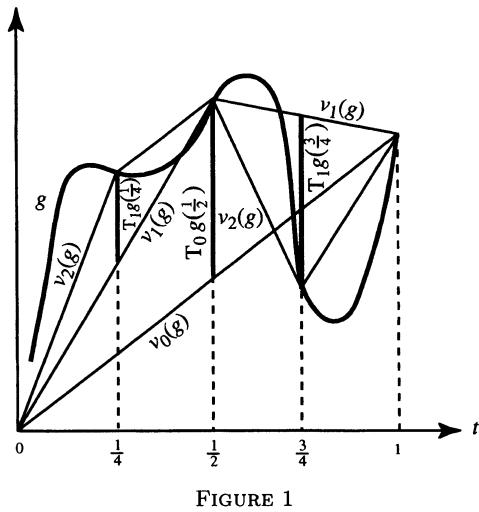
\includegraphics[keepaspectratio]{images/part002_94c2d949.jpg}}

one can then apply Lemma 3 with \(t = \frac{k - 1}{2^n}\) , \(t' = \frac{k}{2^n}\) , whence

\[
\int_ {\Omega} \left| \mathrm{T} _ {n} g \left(\frac {2 k - 1}{2 ^ {n + 1}}\right) \right| ^ {3} d m (g) = \frac {1}{(8 \pi) ^ {1 / 2}} 2 ^ {- \frac {3 n}{2}}.\tag{46}
\]

By (44), we then have

\[
\int_ {\Omega} \| \mathrm{T} _ {n} g \| ^ {3} d m (g) \leqslant \sum_ {k = 1} ^ {2 ^ {n}} \int_ {\Omega} \left| \mathrm{T} _ {n} g \left(\frac {2 k - 1}{2 ^ {n + 1}}\right) \right| ^ {3} d m (g) = \frac {1}{(8 \pi) ^ {1 / 2}} 2 ^ {n} \cdot 2 ^ {- \frac {3 n}{2}},
\]

whence the lemma.

By Lemma 4, the mapping \(\mathbf{T}_n\) of \(\Omega\) into the Banach space \(\mathcal{C}\) belongs to \(\mathrm{L}_{\mathcal{C}}^3 (\Omega ,m)\) and \(\mathrm{N}_3(\mathrm{T}_n)\leqslant \frac{1}{(8\pi)^{1 / 6}} (2^{-1 / 6})^n\) , whence \(\sum_{n = 0}^{\infty}\mathrm{N}_3(\mathrm{T}_n) < + \infty\) . By Prop. 6 of Ch. IV, §3, No.~3, there exists a set \(\Omega_0\subset \Omega\) such that \(\Omega -\Omega_0\) is \(m\) -negligible and such that the series \(\sum_{n = 0}^{\infty}\mathrm{T}_n(g)\) converges absolutely in \(\mathcal{C}\) for every \(g\in \Omega_0\) . One then defines an \(m\) -measurable mapping \(u\) of \(\Omega\) into \(\mathcal{C}\) by

\[
u (g) = \left\{ \begin{array}{c l} \sum_ {n = 0} ^ {\infty} \mathrm{T} _ {n} g = \lim _ {n \to \infty} u _ {n} (g) & \text { for } g \in \Omega_ {0} \\ 0 & \text { for } g \in \Omega - \Omega_ {0}. \end{array} \right.\tag{47}
\]

Since \(u_{n}(g)\) and \(g\) coincide on \(\mathbf{D}_m \subset \mathbf{D}_n\) for \(0 \leqslant m \leqslant n\) , it is immediate that the restriction of \(u(g)\) to \(\mathbf{D}\) is equal to \(g\) for every \(g \in \Omega_0\) .

\begin{enumerate}
\def\labelenumi{\Alph{enumi})}
\setcounter{enumi}{2}
\tightlist
\item
  Construction of a Gaussian measure on \(\mathcal{C}\) :
\end{enumerate}

Let \(w'\) be the bounded measure on \(\mathcal{C}\) that is the image of \(m\) under the \(m\) -measurable mapping \(u: \Omega \to \mathcal{C}\) . We are going to show that \(w'\) is a Gaussian measure on \(\mathcal{C}\) , with variance \(W\) , whence \(w = w'\) . Denote by \(\mathcal{D}\) the linear subspace of \(\mathcal{M}^1\) generated by the measures \(\varepsilon_t\) for \(t\) running over \(D\) .

Lemma 5. --- For every measure \(\mu \in \mathcal{D}\) ,

\[
\int_ {\mathcal {C}} e ^ {i \langle f, \mu \rangle} d w ^ {\prime} (f) = e ^ {- W (\mu) / 2}.\tag{48}
\]

Set \(\mu=c_{1}\varepsilon_{t_{1}}+c_{2}\varepsilon_{t_{2}}+\cdots+c_{n}\varepsilon_{t_{n}}\) with \(t_{1},\ldots,t_{n}\) in D and \(c_{1},\ldots,c_{n}\) in R. For every \(g\in\Omega_{0}\) , the function \(u(g)\) coincides with g on D; therefore

\[
\langle u (g), \mu \rangle = \sum_ {j = 1} ^ {n} c _ {j} g (t _ {j}) \quad (g \in \Omega_ {0}).\tag{49}
\]

Also,

\[
\mathrm{W} (\mu) = \sum_ {j, k = 1} ^ {n} c _ {j} c _ {k} \inf (t _ {j}, t _ {k}),\tag{50}
\]

and, since m is the Gaussian measure on \(\Omega\) with covariance M, and \(\Omega - \Omega_{0}\) is m-negligible, we have

\[
\int_ {\Omega_ {0}} e ^ {i \sum_ {j = 1} ^ {n} c _ {j} g (t _ {j})} d m (g) = \exp \Big (- \frac {1}{2} \sum_ {j, k = 1} ^ {n} c _ {j} c _ {k} \inf (t _ {j}, t _ {k}) \Big).\tag{51}
\]

Now, \(\Omega - \Omega_0\) is \(m\) -negligible and \(w' = u(m)\) ; it follows that

\[
\int_ {\mathcal {C}} e ^ {i \langle f, \mu \rangle} d w ^ {\prime} (f) = \int_ {\Omega_ {0}} e ^ {i \langle u (g), \mu \rangle} d m (g).\tag{52}
\]

The formula (48) follows immediately from the formulas (49) to (52).

Lemma 6. --- Let \(\mu \in \mathcal{M}^1\) . There exists a sequence of measures \(\mu_n \in \mathcal{D}\) such that \(\mu(f) = \lim_{n \to \infty} \mu_n(f)\) for all \(f \in \mathcal{C}\) and \(\mathrm{W}(\mu) = \lim_{n \to \infty} \mathrm{W}(\mu_n)\) .

Let \(I = [0,1]\) . The space \(\mathcal{M}^1\) of bounded measures on \(T = ]0,1]\) will be identified with the subspace of \(\mathcal{M}(I)\) formed by the measures that place no weight at 0. \(^{(3)}\) We equip \(\mathcal{M}(I)\) with the vague topology. The mapping \(t \mapsto \varepsilon_t\) of I into \(\mathcal{M}(I)\) is continuous (Ch. III, §1, No.~9, Prop. 13); since D is dense in I, the closure \(\overline{\mathcal{D}}\) of \(\mathcal{D}\) contains all of the point measures. Let A be the set of measures \(\nu \in \mathcal{D}\) such that \(\| \nu \| \leqslant \| \mu \|\) ; the measure \(\mu\) is in the closure of A (Ch. III, §2, No.~4, Cor. 1 of Th. 1). The set A is relatively compact in \(\mathcal{M}(I)\) (Ch. III, §1, No.~9, Prop. 15) and the compact subsets of \(\mathcal{M}(I)\) are metrizable (TVS, III, §3, No.~4, Cor. 2 of Prop. 6, \(^{(4)}\) and GT, X, §3, No.~3, Th. 1). Therefore there exists a sequence of measures \(\mu_n \in A\) converging to \(\mu\) in \(\mathcal{M}(I)\) . Since \(\mathcal{C}\) is identified with the subspace of continuous functions on I zero at the origin, we have \(\mu(f) = \lim_{n \to \infty} \mu_n(f)\) for all \(f \in \mathcal{C}\) . Moreover, since \(\mathcal{C}(I) \otimes \mathcal{C}(I)\) is dense in the normed space \(\mathcal{C}(I \times I)\) (Ch. III, §4, No.~1, Lemma 1), the relations \(\lim_{n \to \infty} \mu_n = \mu\) and \(\| \mu_n \| \leqslant \| \mu \|\) imply that \(\lim_{n \to \infty} (\mu_n \otimes \mu_n) = \mu \otimes \mu\) (Ch. III, §1, No.~10, Prop. 17); since the measures \(\mu_n\) and \(\mu\) place no weight at 0, we have

\[
\begin{array}{r} \mathrm{W} (\mu_ {n}) = \int_ {\mathrm{I}} \int_ {\mathrm{I}} \inf (t, t ^ {\prime}) d \mu_ {n} (t) d \mu_ {n} (t ^ {\prime}), \\ \mathrm{W} (\mu) = \int_ {\mathrm{I}} \int_ {\mathrm{I}} \inf (t, t ^ {\prime}) d \mu (t) d \mu (t ^ {\prime}), \end{array}
\]

whence \(\lim_{n\to \infty}\mathrm{W}(\mu_n) = \mathrm{W}(\mu)\) .

It remains to prove that the Fourier transform of \(w'\) is equal to \(e^{-\mathbf{W}/2}\) . Let \(\mu \in \mathcal{M}^1\) ; choose measures \(\mu_n \in \mathcal{D}\) as in Lemma 6. The measure \(w'\) is bounded, and \(|e^{i\langle f,\mu_n\rangle}| = 1\) for all \(n\) ; Lemma 5 and Lebesgue's convergence theorem (Ch. IV, §4, No.~3, Th. 2) then imply

\[
\begin{array}{r l} \int_ {\mathcal {C}} e ^ {i \langle f, \mu \rangle} d w ^ {\prime} (f) & = \lim _ {n \to \infty} \int_ {\mathcal {C}} e ^ {i \langle f, \mu_ {n} \rangle} d w ^ {\prime} (f) \\ & = \lim _ {n \to \infty} e ^ {- \mathrm{W} (\mu_ {n}) / 2} = e ^ {- \mathrm{W} (\mu) / 2}. \end{array}\tag{Q.E.D.}
\]

The measure \(w\) on \(\mathcal{C}\) whose Fourier transform is equal to \(e^{-\mathrm{W} / 2}\) is called the Wiener measure on \(\mathcal{C}\) .

Remark. --- For every semi-open interval \(J = ]a, b]\) contained in \(T\) , let us set \(l(J) = b - a\) (the length of \(J\) ) and denote by \(A_J\) the linear form \(f \mapsto f(b) - f(a)\) on \(\mathcal{C}\) . It can be shown that the Wiener measure is characterized by the following property:

Let \(J_{1},\ldots,J_{n}\) be semi-open intervals contained in T and pairwise disjoint. The image of the measure w under the linear mapping \(f\mapsto\left(\mathrm{A}_{\mathrm{J}_{1}}(f),\ldots,\mathrm{A}_{\mathrm{J}_{n}}(f)\right)\) of C into \(R^{n}\) is equal to \(\gamma_{a_{1}}\otimes\cdots\otimes\gamma_{a_{n}}\) with \(a_{i}=l(J_{i})^{1/2}\) for \(1\leqslant i\leqslant n\) .

